\section{Uæltet brød}
Lækkert lyst, tæt og svampet brød, som ikke skal æltes. Overhovedet.

\subsection{Ingredienser}
Efter at lave konsulteret internettet lader dette til at være opskriften på sejr.

\begin{multicols}{2}
	\begin{itemize}
		\item Hvedemel $\times$ 400g
		\item Gær $\times$ 1g
		\item Salt $\times$ 10g
		\item Sukker $\times$ 10g
		\item Vand $\times$ 300g
		\item En 6. ting, som gør listen pæn.
	\end{itemize}
\end{multicols}

Vandet skal være rumtemperatur. Så tjek det, før du dræber gæret!

\subsection{Grej}
Denne gang skal vi bruge noget ikke alle har - så tjek at du har følgende.

\begin{itemize}
	\item En rimelig stor støbejernsgryde med låg.
\end{itemize}

\subsection{Fremgangsmåde, Dag 1}
Vi ælter ingenting, men tingene skal nu blandes alligevel. Livet er hårdt.

\paragraph*{1. Bland de våde sager}
Der er ikke så meget andet at sige. Brug 10 sekunder og værdsæt at du næsten er færdig.

\paragraph*{2. Tilsæt de tørre sager}
Bland det hele indtil det hænger sammen og der ikke meget mel på siderne af skålen. Hvis det tager dig mere end 30 sekunder prøver du for hårdt. Se Figur~\ref{fig:no-knead-bread-after-not-kneading} på Side~\pageref{fig:no-knead-bread-after-not-kneading} du er i tvivl.

\paragraph*{3. Smid låg på}
Det skal hvile i 12 til 24 timer, eller indtil det er fordoblet i størrelse. Tak for i dag - vi ses i morgen.

\subsection{Fremgangsmåde, Dag 2}
Vores baby er nu (forhåbentligt) vokset til mindst dobbelt størrelse og har pruttet hele natten - hvilket gerne skulle kunne duftes.

\paragraph*{4. Forvarm hvad forvarmes kan}
Du tænder ovnen på alt hvad den trække og smider din støbejernsfætter ind. Cirka 50 minutter senere forsætter du herfra.

\paragraph*{5. Fold dejen ind på sig selv}
Hør nu efter. Det bliver et klisterhelvede. Der skal masser af mel på bordet! Den skal \textbf{ikke} (!) æltes, men bare lige foldes nogle gange. Gør det nogle få gange indtil den ligner en pæn dej med en stram overflade.

\paragraph*{6. Forbered afgang mod ovn}
Ved at smide den på et velmelet stykke bagepapir og sprøjt den gavmildt til med vand. Sænk den så forsigtigt ned i din støbejernsgryde (pas nu på pølserne). Sæt læg på og efterlad i ovnen i 30 minutter før næste inspektion.

\paragraph*{7. La' det lig'}
I mindst en time før du fucker med brødet. Alt er spildt hvis du rør den før - det skal ikke diskuteres.

\begin{figure}[h]
	\centering
	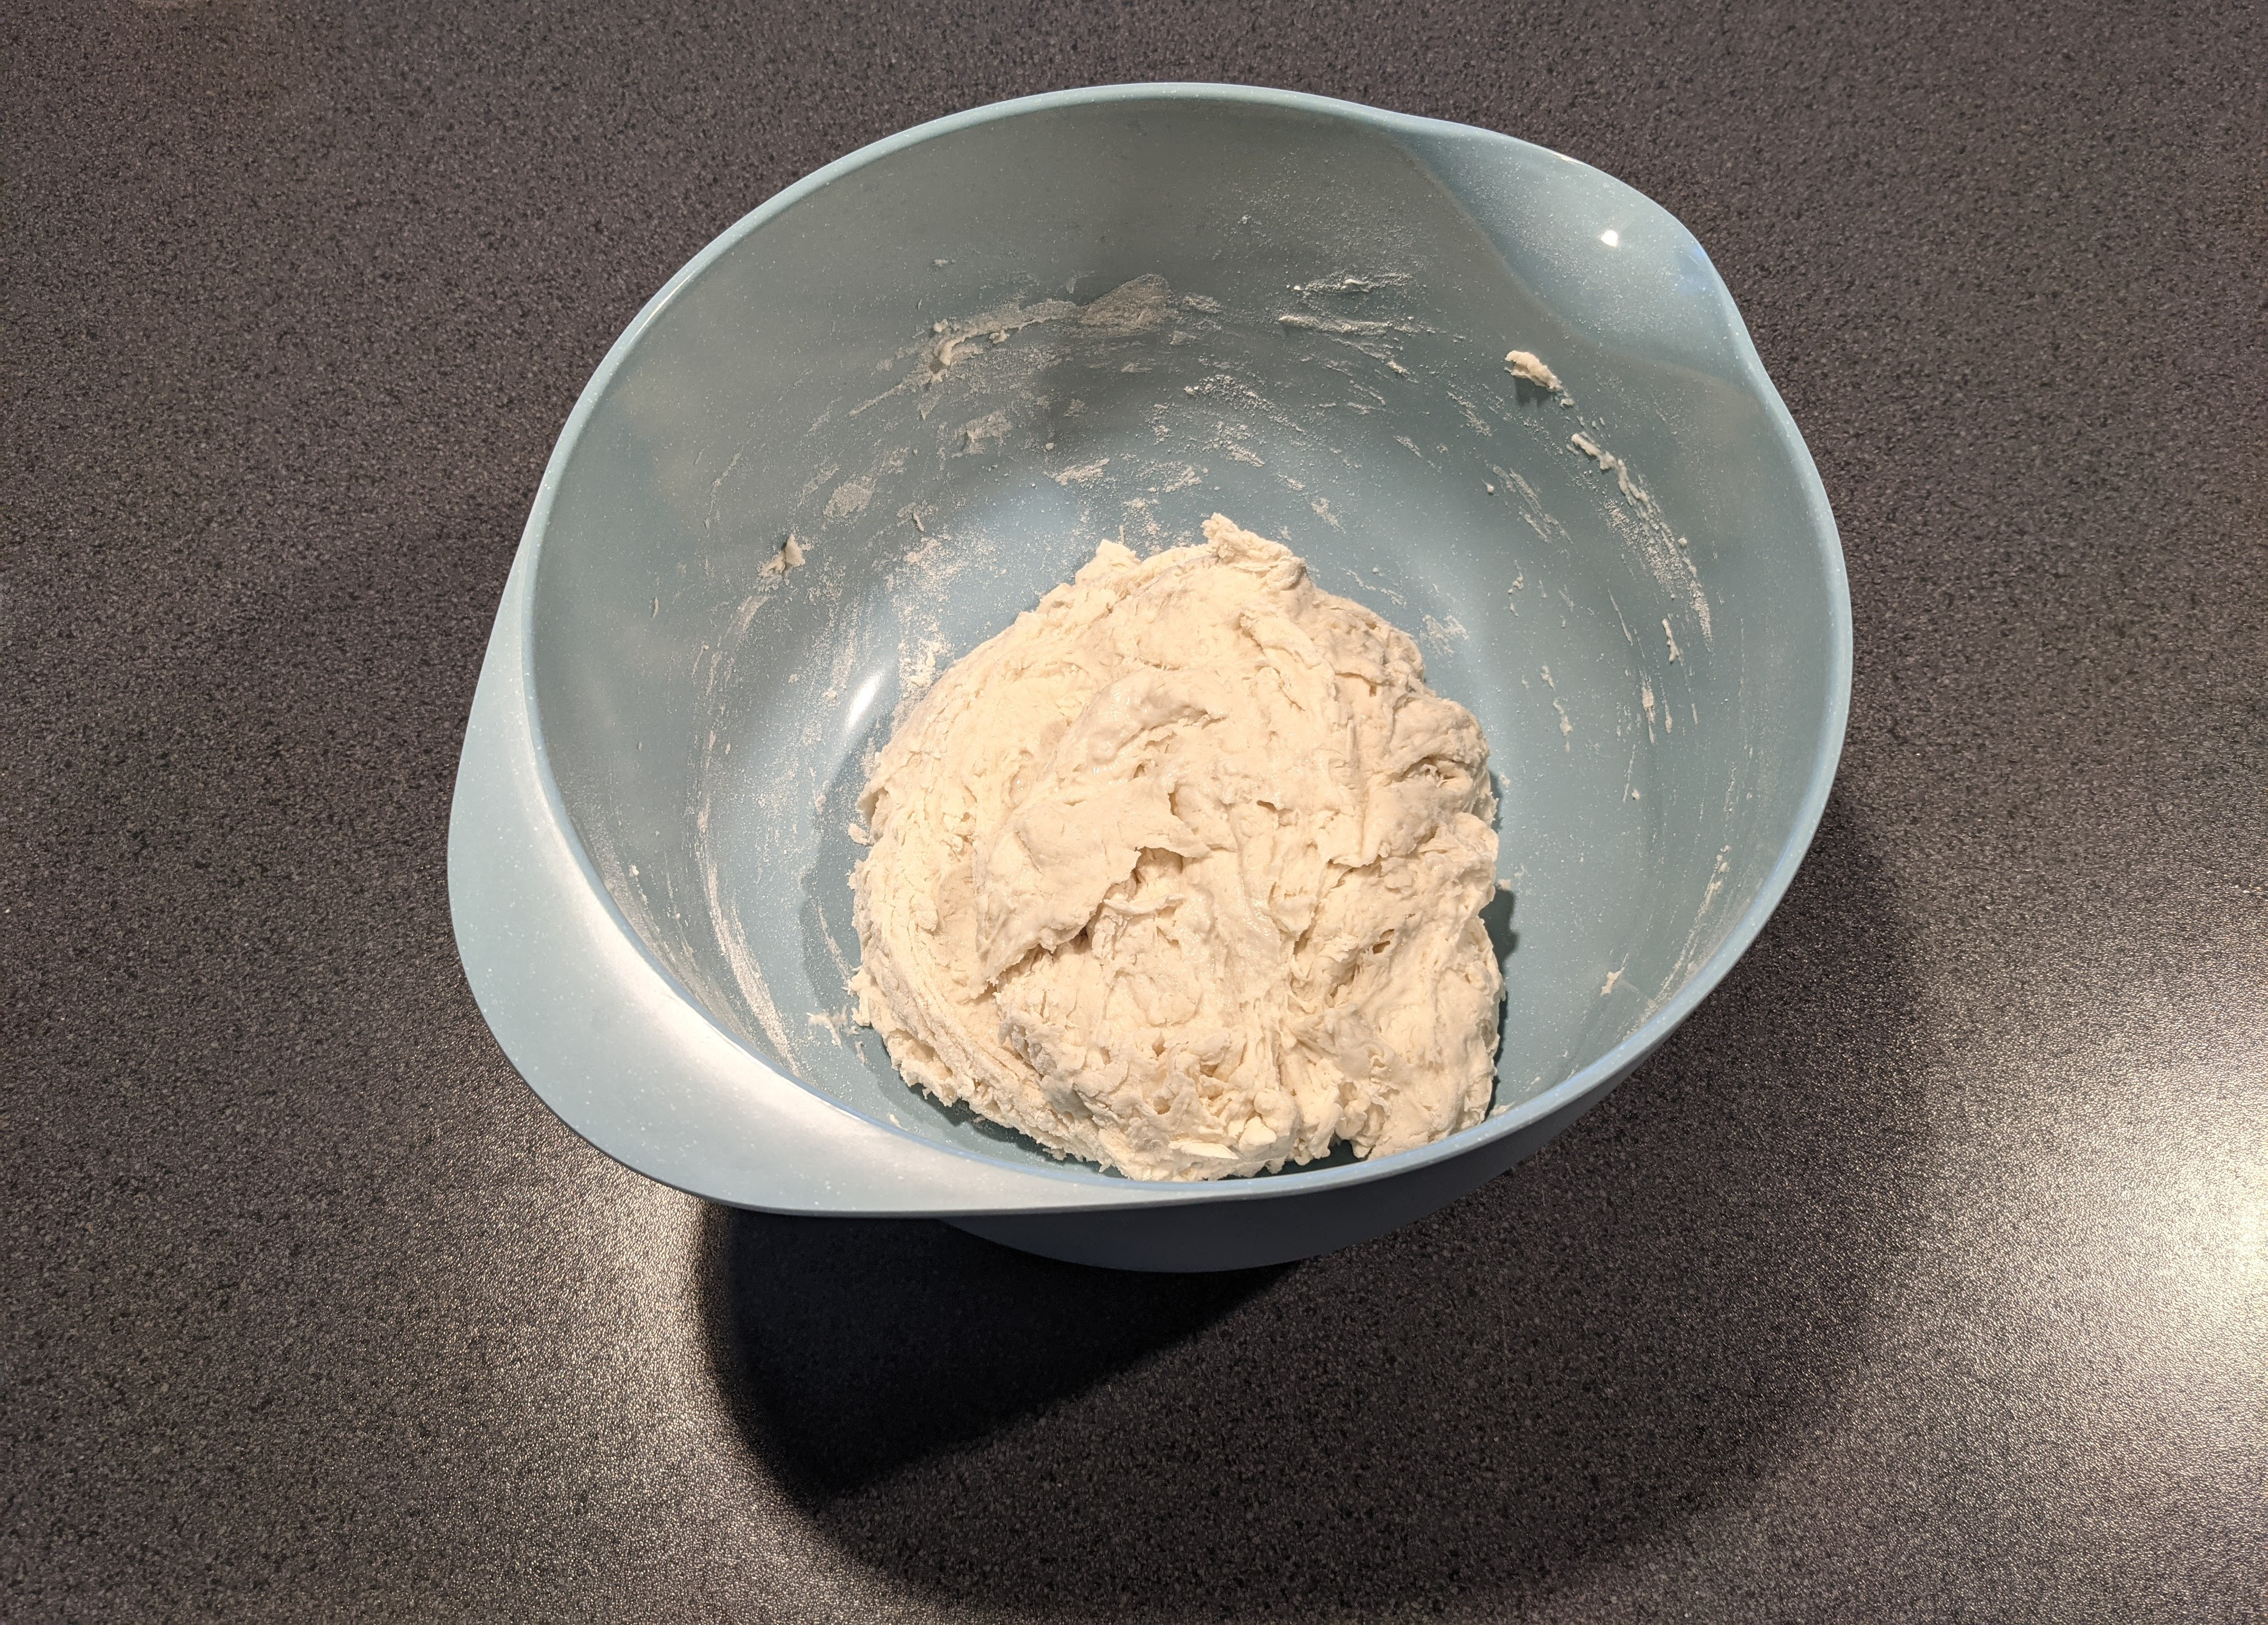
\includegraphics[width=\linewidth]{figs/no-knead-bread-after-not-kneading}
	\caption{Uæltet dej efter ikke at være blevet æltet.}
	\label{fig:no-knead-bread-after-not-kneading}
\end{figure}
